\section{Project Design}

\subsection{Real-World Scenario}

Urban Scout was designed around a realistic tourism scenario in which short-term visitors need quick access to multiple types of local information while moving through a city. In practice, tourists often rely on several disconnected platforms to plan their day. A traveler may use one service to find landmarks, another to locate restaurants, another to check transit schedules, and another to search for local events, closures, or safety concerns. This separation of information creates unnecessary friction, especially for users who are unfamiliar with the city and need fast, location-aware decisions.

The project models a tourism support system for Seoul, with data organized into major regions such as Downtown Seoul, Gangnam, and Hongdae. These regions help structure the application and allow the system to connect transit, destinations, local updates, and user activity in a meaningful way. By placing all of this information in one relational database, Urban Scout reduces context switching and allows users to interact with related information through a single interface.

\subsection{User Groups}

The system was designed for two primary categories of users: regular users and administrators.

\boldheading{Regular Users}

Regular users represent tourists or visitors using the platform to explore the city and organize their travel plans. Their main goals are to find places of interest, understand how to move between locations, stay informed about local conditions, and build simple itineraries.

The system allows regular users to:
\begin{itemize}
    \item log in using a seeded email account
    \item browse regions and subscribe to regions of interest
    \item view places such as landmarks, eateries, and transit stations
    \item access transit-related information for selected stations
    \item read region-based news and safety alerts
    \item submit incident reports connected to a region
    \item create and manage itineraries
    \item view their own submitted reports
\end{itemize}

These functions were chosen because they reflect common tourist needs: discovering what exists in an area, deciding where to go, understanding how to get there, and staying aware of ongoing events or hazards.

\boldheading{Administrators}

Administrators represent trusted system managers who maintain local updates and review user-submitted reports. Their role supports the reliability and usefulness of the platform.

The system allows administrators to:
\begin{itemize}
    \item log in through the admin interface
    \item access protected admin pages
    \item review incident reports submitted by users
    \item verify or update the status of reports
    \item create and manage regional news posts
    \item contribute to the safety and information layer of the application
    \item add new places (landmarks, eateries, transit stations) to a region
    \item add and remove transit routes and link station-vehicle pairs as stops on a route
\end{itemize}

This user group was included because the project is not only a read-only guide. It also models a system where information can be maintained and moderated, making the application more realistic and dynamic.

\subsection{Core Design Goals}

Several design goals guided the structure of the project.

\boldheading{Unified Information Access}

The main goal was to combine multiple categories of travel-related data into one database-backed system. Instead of forcing users to mentally connect unrelated apps, the system was designed to connect places, regions, transit, safety information, and itineraries through explicit relationships in the schema.

\boldheading{Relational Integration}

A central goal of the database design was to ensure that the major entities were meaningfully linked. For example:
\begin{itemize}
    \item each place belongs to a region
    \item transit stations are represented as places
    \item nearby places can be connected to stations
    \item news posts are associated with regions
    \item safety alerts are attached to news posts
    \item incident reports are tied to both users and regions
    \item itinerary items reference specific places
\end{itemize}

This relational structure is one of the most important aspects of the project because it supports the ``unified assistant'' concept at the data level, not just in the user interface.

\boldheading{Mobile-Friendly Interaction}

Because tourists are likely to use the system while moving through a city, the interface was designed with a mobile-first approach. Navigation was kept simple, page content was organized into cards and lists, and the app was built to work well on smaller screens. This goal influenced both the frontend layout and the choice to keep user actions straightforward.

\boldheading{Role-Based Access}

The project also aimed to support different types of users without overcomplicating the experience. Regular users and administrators have different responsibilities, so the system includes role-based access to ensure that only administrators can perform moderation tasks such as managing news or verifying reports.

\subsection{Major Entities and Relationships}

The ER design centers around a set of entities that model the tourism scenario.

\boldheading{Region}

A \texttt{Region} represents a major area of the city. Regions organize places, news, and user subscriptions. They help group related information and allow region-based browsing and filtering.

\boldheading{Place}

A \texttt{Place} is a general entity used to represent locations relevant to the user. This entity is specialized into subtypes such as landmarks, eateries, and transit stations. This design avoids duplication while allowing each subtype to store its own attributes.

\boldheading{Landmark, Eatery, and TransitStation}

These entities specialize \texttt{Place}:
\begin{itemize}
    \item \texttt{Landmark} stores landmark-specific details such as type and hours
    \item \texttt{Eatery} stores dining-related details such as average cost
    \item \texttt{TransitStation} stores transit-specific details such as station code
\end{itemize}

This specialization structure was chosen to reflect the fact that these entities share common location data but also have distinct properties.

\boldheading{PublicTransit and TransitRoute}

\texttt{PublicTransit} represents specific transit services such as subway lines, buses, or trains. \texttt{TransitRoute} provides route-level information such as route names and service hours. The relationships among routes, stations, and transit services allow the application to display schedules and station-level service information.

\boldheading{NewsPost and SafetyAlert}

\texttt{NewsPost} stores regional updates and local information. \texttt{SafetyAlert} is modeled as a weak entity attached to a news post, allowing a single news item to contain one or more specific alerts. This is useful for representing situations where a larger event has multiple localized impacts.

\boldheading{IncidentReport}

An \texttt{IncidentReport} stores user-submitted safety or hazard information. Each report is linked to the user who submitted it and the region in which it occurred. This allows the system to collect user-generated information while still preserving geographic context.

\boldheading{Itinerary and ItineraryItem}

\texttt{Itinerary} stores a user's travel plan. \texttt{ItineraryItem} is a weak entity that represents individual scheduled items within an itinerary. Each itinerary item can reference a place, allowing users to connect planned activities to actual destinations in the database.

\subsection{Relationship Design}

Several relationships were included to capture how the different entities interact in practice.

\begin{itemize}
    \item A user can subscribe to one or more regions.
    \item A user can create one or more itineraries.
    \item An itinerary includes one or more itinerary items.
    \item An itinerary item references a place.
    \item A place belongs to a region.
    \item An admin is assigned to a region.
    \item An admin can verify incident reports.
    \item A news post is published for a region.
    \item A news post can contain safety alerts.
    \item A transit route serves a transit station.
    \item A place can be associated with a nearby transit station through a proximity relationship.
\end{itemize}

These relationships were intentionally chosen to support the features visible in the interface. They are not abstract additions, each one supports either browsing, filtering, reporting, route display, or planning.

\subsection{ER Diagram}

The ER diagram for Urban Scout reflects the complete conceptual design of the project. It includes strong entities, weak entities, specialization, and many-to-many relationships resolved through associative structures.

The most notable features of the ER design are:
\begin{itemize}[nosep]
    \item specialization from \texttt{Place} into \texttt{Landmark}, \texttt{Eatery}, and \texttt{TransitStation}
    \item weak entity treatment of \texttt{SafetyAlert}
    \item weak entity treatment of \texttt{ItineraryItem}
    \item associative relationships connecting users to regions, places to stations, and routes to stations and transit services
\end{itemize}
\nopagebreak[4]

\begin{figure}[H]
    \centering
    \IfFileExists{figures/eer.png}{%
        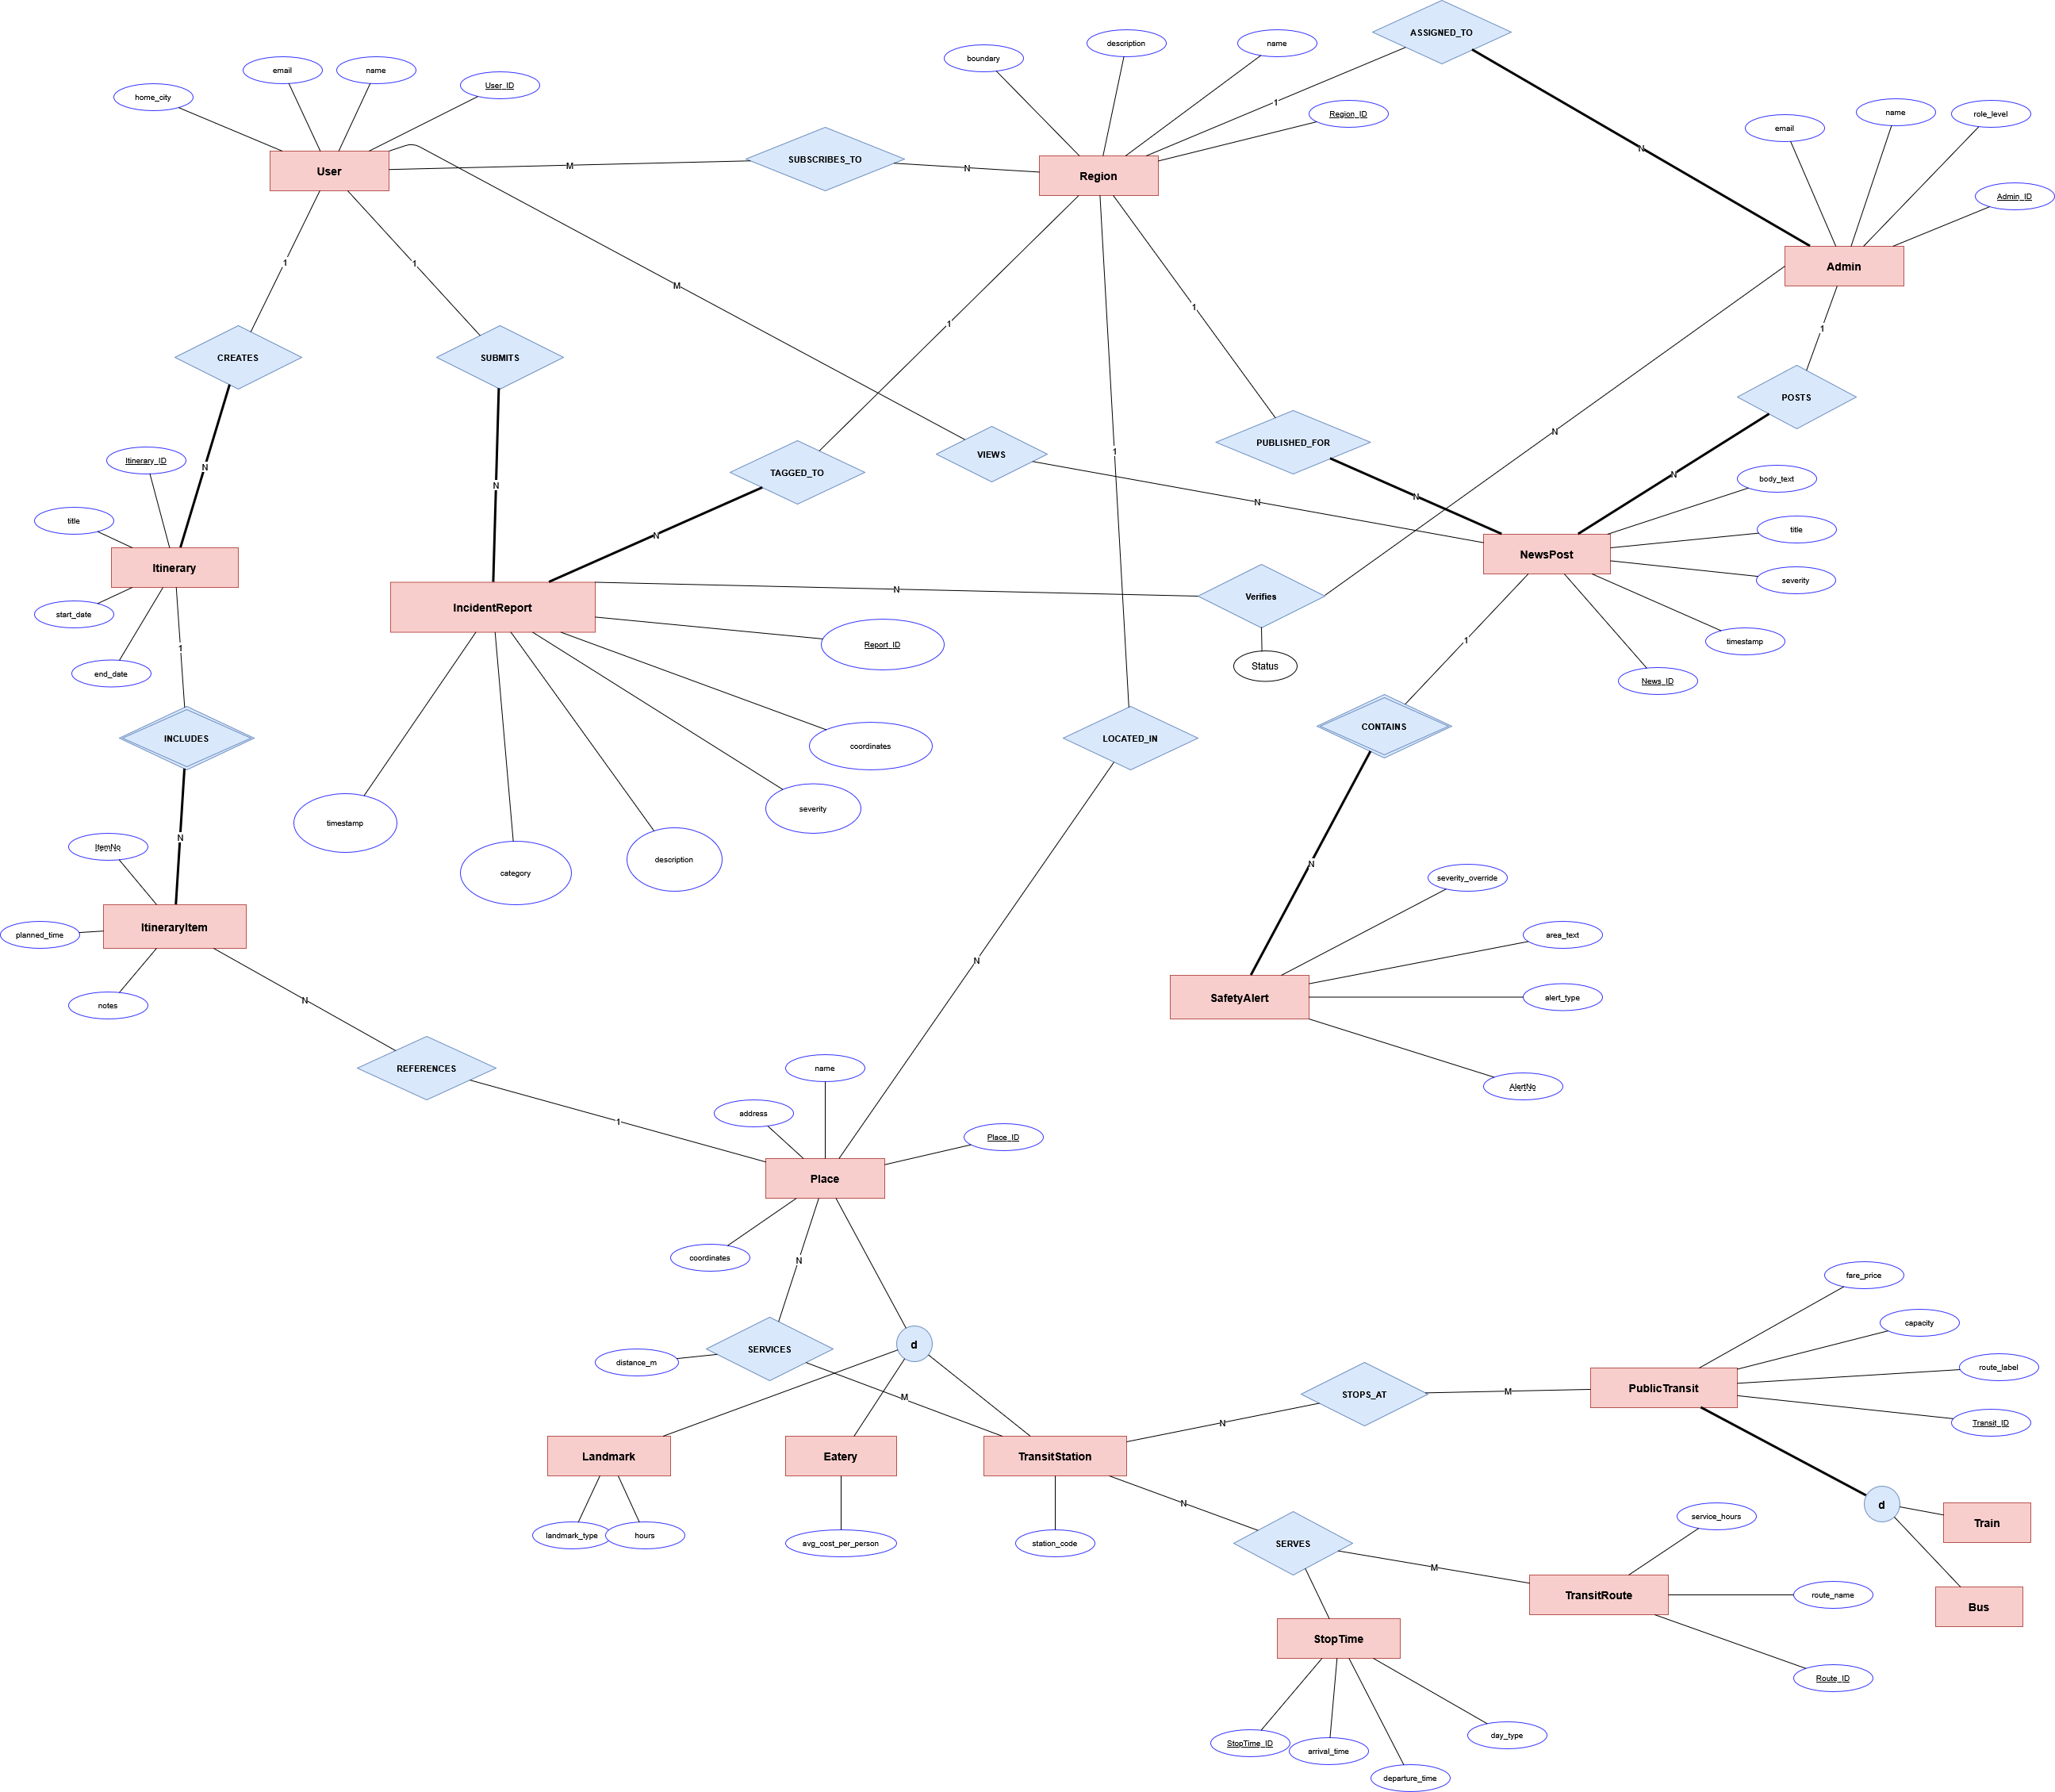
\includegraphics[width=\textwidth,keepaspectratio]{figures/eer.png}%
    }{%
        \fbox{\parbox{0.95\textwidth}{\centering\vspace{3cm}\textbf{Placeholder for EER diagram}\\\vspace{0.3cm}This figure will show the Extended Entity-Relationship diagram for Urban Scout, including all 16 entity types, the two specialization hierarchies (\texttt{Place} and \texttt{PublicTransit}), the two weak entities (\texttt{SafetyAlert} and \texttt{ItineraryItem}), and all relationship types.\\\vspace{0.3cm}\texttt{figures/eer.png}\vspace{3cm}}}%
    }
    \caption{Extended Entity-Relationship diagram for Urban Scout.}
    \label{fig:eer}
\end{figure}

No structural changes were made to the schema between the presentation and this final report. Features that were not yet wired up at presentation time, such as admin-side place management and admin-side transit route management, were already represented in the EER and only required interface implementation. The diagram above matches the version shown during the demo.

\subsection{Design Assumptions}

The following assumptions guided the conceptual and relational design of Urban Scout. They clarify how the schema enforces identity, participation, and referential constraints across the major entities.

\begin{enumerate}
    \item \texttt{USER(UserID)} uniquely identifies each user account.
    \item \texttt{ADMIN(AdminID)} uniquely identifies each admin.
    \item Admins are the only entities referenced by \texttt{NEWS\_POST.AdminID}, enforcing that only admins can create news content.
    \item Each \texttt{ADMIN} tuple contains a foreign key \texttt{RegionID} referencing \texttt{REGION(RegionID)}, enforcing that each admin is assigned to exactly one region and that admins can only manage content for their assigned region.
    \item \texttt{PLACE(PlaceID)} uniquely identifies each place.
    \item \texttt{PLACE} contains a foreign key \texttt{RegionID} referencing \texttt{REGION(RegionID)}, enforcing that each place belongs to exactly one region and cannot belong to multiple regions.
    \item The specialization of \texttt{PLACE} into \texttt{LANDMARK}, \texttt{EATERY}, and \texttt{TRANSIT\_STATION} is disjoint and partial. Disjoint means a given \texttt{PlaceID} can appear in at most one subclass table. Partial means a \texttt{PlaceID} may exist in \texttt{PLACE} without appearing in any subclass relation.
    \item Each subclass relation (\texttt{LANDMARK}, \texttt{EATERY}, \texttt{TRANSIT\_STATION}) uses \texttt{PlaceID} as both its primary key and a foreign key referencing \texttt{PLACE(PlaceID)}.
    \item \texttt{NEWS\_POST(NewsID)} uniquely identifies each news post.
    \item \texttt{NEWS\_POST.RegionID} is a foreign key referencing \texttt{REGION(RegionID)}, enforcing that each news post is published for exactly one region while a region may have multiple news posts.
    \item \texttt{SAFETY\_ALERT} is a weak entity. It is identified by the composite primary key \texttt{(NewsID, AlertNo)}, where \texttt{NewsID} is a foreign key referencing \texttt{NEWS\_POST(NewsID)}. Total participation is enforced because \texttt{NewsID} is part of the primary key and cannot be null.
    \item \texttt{INCIDENT\_REPORT(Report\_ID)} uniquely identifies each incident report.
    \item \texttt{INCIDENT\_REPORT.UserID} is a foreign key referencing \texttt{USER(UserID)}, enforcing that each report is submitted by exactly one user while a user may submit multiple reports.
    \item \texttt{INCIDENT\_REPORT.RegionID} is a foreign key referencing \texttt{REGION(RegionID)}, enforcing that each report is associated with exactly one region while a region may have multiple reports.
    \item The many-to-many relationship between \texttt{USER} and \texttt{REGION} is resolved by \texttt{SUBSCRIPTION(UserID, RegionID)}, which uses a composite primary key where both attributes are foreign keys referencing their respective parent relations.
    \item \texttt{TRANSIT\_ROUTE(RouteID)} uniquely identifies each transit route.
    \item \texttt{STOP\_TIME(RouteID, PlaceID, arrival\_time)} has a composite primary key. \texttt{RouteID} references \texttt{TRANSIT\_ROUTE(RouteID)} and \texttt{PlaceID} references \texttt{TRANSIT\_STATION(PlaceID)}. The relation also stores schedule attributes such as \texttt{arrival\_time}, \texttt{departure\_time}, and \texttt{sequence\_number}.
    \item Transit station to place proximity is modeled as a stored relationship attribute (for example, \texttt{walking\_distance}) and does not require a separate associative relation.
    \item All foreign key attributes enforce referential integrity constraints. A foreign key value must reference an existing primary key value, and primary key attributes cannot be null.
\end{enumerate}

\subsection{Design Rationale}

The final design reflects a balance between realism and project scope. The system is complex enough to demonstrate meaningful database concepts such as specialization, weak entities, role-based users, and many-to-many relationships, but still focused enough to be implemented within a course project. The schema was designed not only to satisfy database design requirements, but also to support visible frontend functionality.

As a result, Urban Scout is more than a collection of unrelated tables. It is a relational system in which data about places, transit, alerts, reports, and travel plans can be combined to support a coherent user experience.
